% =============================================================================================
% 3 Results. Descriptive only; each paragraph <= 100 words. Orange = repeat-0 only / pending.
% Sources: results/results_all.csv, deltas.csv, temporal_*.csv, expB_*.csv, interp_*.csv (2026-10-24)
% =============================================================================================
\section{Results}
\label{sec:results}

\paragraph{Main model.}
A random model's AUPRC equals the event rate (5.5\%), so we report AUPRC with its lift (AUPRC $\div$ event rate). All
numbers are internal nested-CV estimates. The clinical elastic net reached AUPRC 0.366 (95\% CI 0.281--0.487; lift 6.7)
and AUROC 0.807 (0.771--0.868). Frozen DenseNet PCA-32 embeddings added little (AUPRC 0.386; $\Delta$ $+0.020$, $-0.049$
to $0.076$). The cross-fitted pixel logit raised AUPRC to 0.552 (0.472--0.685; lift 10.1) and AUROC to 0.892
(0.861--0.936): $\Delta$AUPRC $+0.203$ (0.121--0.287), $\Delta$AUROC $+0.078$ (0.042--0.121). LightGBM, EBM and the
FT-Transformer did not exceed M0 (all $\Delta$ CIs cross zero; Fig.~\ref{fig:models}).

\paragraph{Threshold metrics.}
At the 10\% risk threshold of the decision curve, the fusion model flagged 8.9\% of hips. It found 62\% of
replacements with precision 0.38 and MCC 0.45, against 54\%, 0.21 and 0.27 for M0 (Table~\ref{tab:threshold}). At
a fixed workload, the top 10\% of hips, sensitivity rose from 0.47 to 0.65. The three tabular comparators and the
FT-Transformer were within 0.03 MCC of M0. The image head alone reached MCC 0.44, close to the fusion model.

\begin{table}[!tbp]
  \centering
  \caption{\textbf{Threshold metrics at two operating points.} Left: calibrated risk $\ge$10\%, the threshold of the
  decision curve (the share of hips flagged depends on calibration). Right: the 10\% of hips with the highest risk (a
  fixed workload of about 170 hips, independent of calibration). Sensitivity, precision (positive predictive value) and
  Matthews correlation coefficient (MCC) are computed per repeat on pooled out-of-fold predictions and averaged over five
  repeats; the event rate is 5.5\%. The image head is calibrated on its cross-fitted inner predictions.}
  \label{tab:threshold}
  \small
  \setlength{\tabcolsep}{4pt}
  \begin{tabular}{@{}lccccccc@{}}
    \toprule
    & \multicolumn{4}{c}{Risk $\ge$ 10\%} & \multicolumn{3}{c}{Top 10\% of hips} \\
    \cmidrule(lr){2-5}\cmidrule(l){6-8}
    Model & Flagged & Sens. & Prec. & MCC & Sens. & Prec. & MCC \\
    \midrule
    M0 elastic net (clinical) & 14\% & 0.54 & 0.20 & 0.27 & 0.47 & 0.26 & 0.30 \\
    M1 LightGBM & 14\% & 0.54 & 0.21 & 0.28 & 0.48 & 0.26 & 0.30 \\
    M1b EBM & 13\% & 0.52 & 0.21 & 0.27 & 0.46 & 0.25 & 0.28 \\
    M2 FT-Transformer & 11\% & 0.48 & 0.23 & 0.28 & 0.46 & 0.25 & 0.29 \\
    M3 image head (pixels only) & 7\% & 0.54 & 0.41 & 0.44 & 0.61 & 0.34 & 0.41 \\
    \textbf{M0 + pixel logit (final)} & \textbf{9\%} & \textbf{0.62} & \textbf{0.38} & \textbf{0.45} & \textbf{0.65} & \textbf{0.35} & \textbf{0.44} \\
    \bottomrule
  \end{tabular}
\end{table}


\begin{figure}[!tbp]
  \centering
  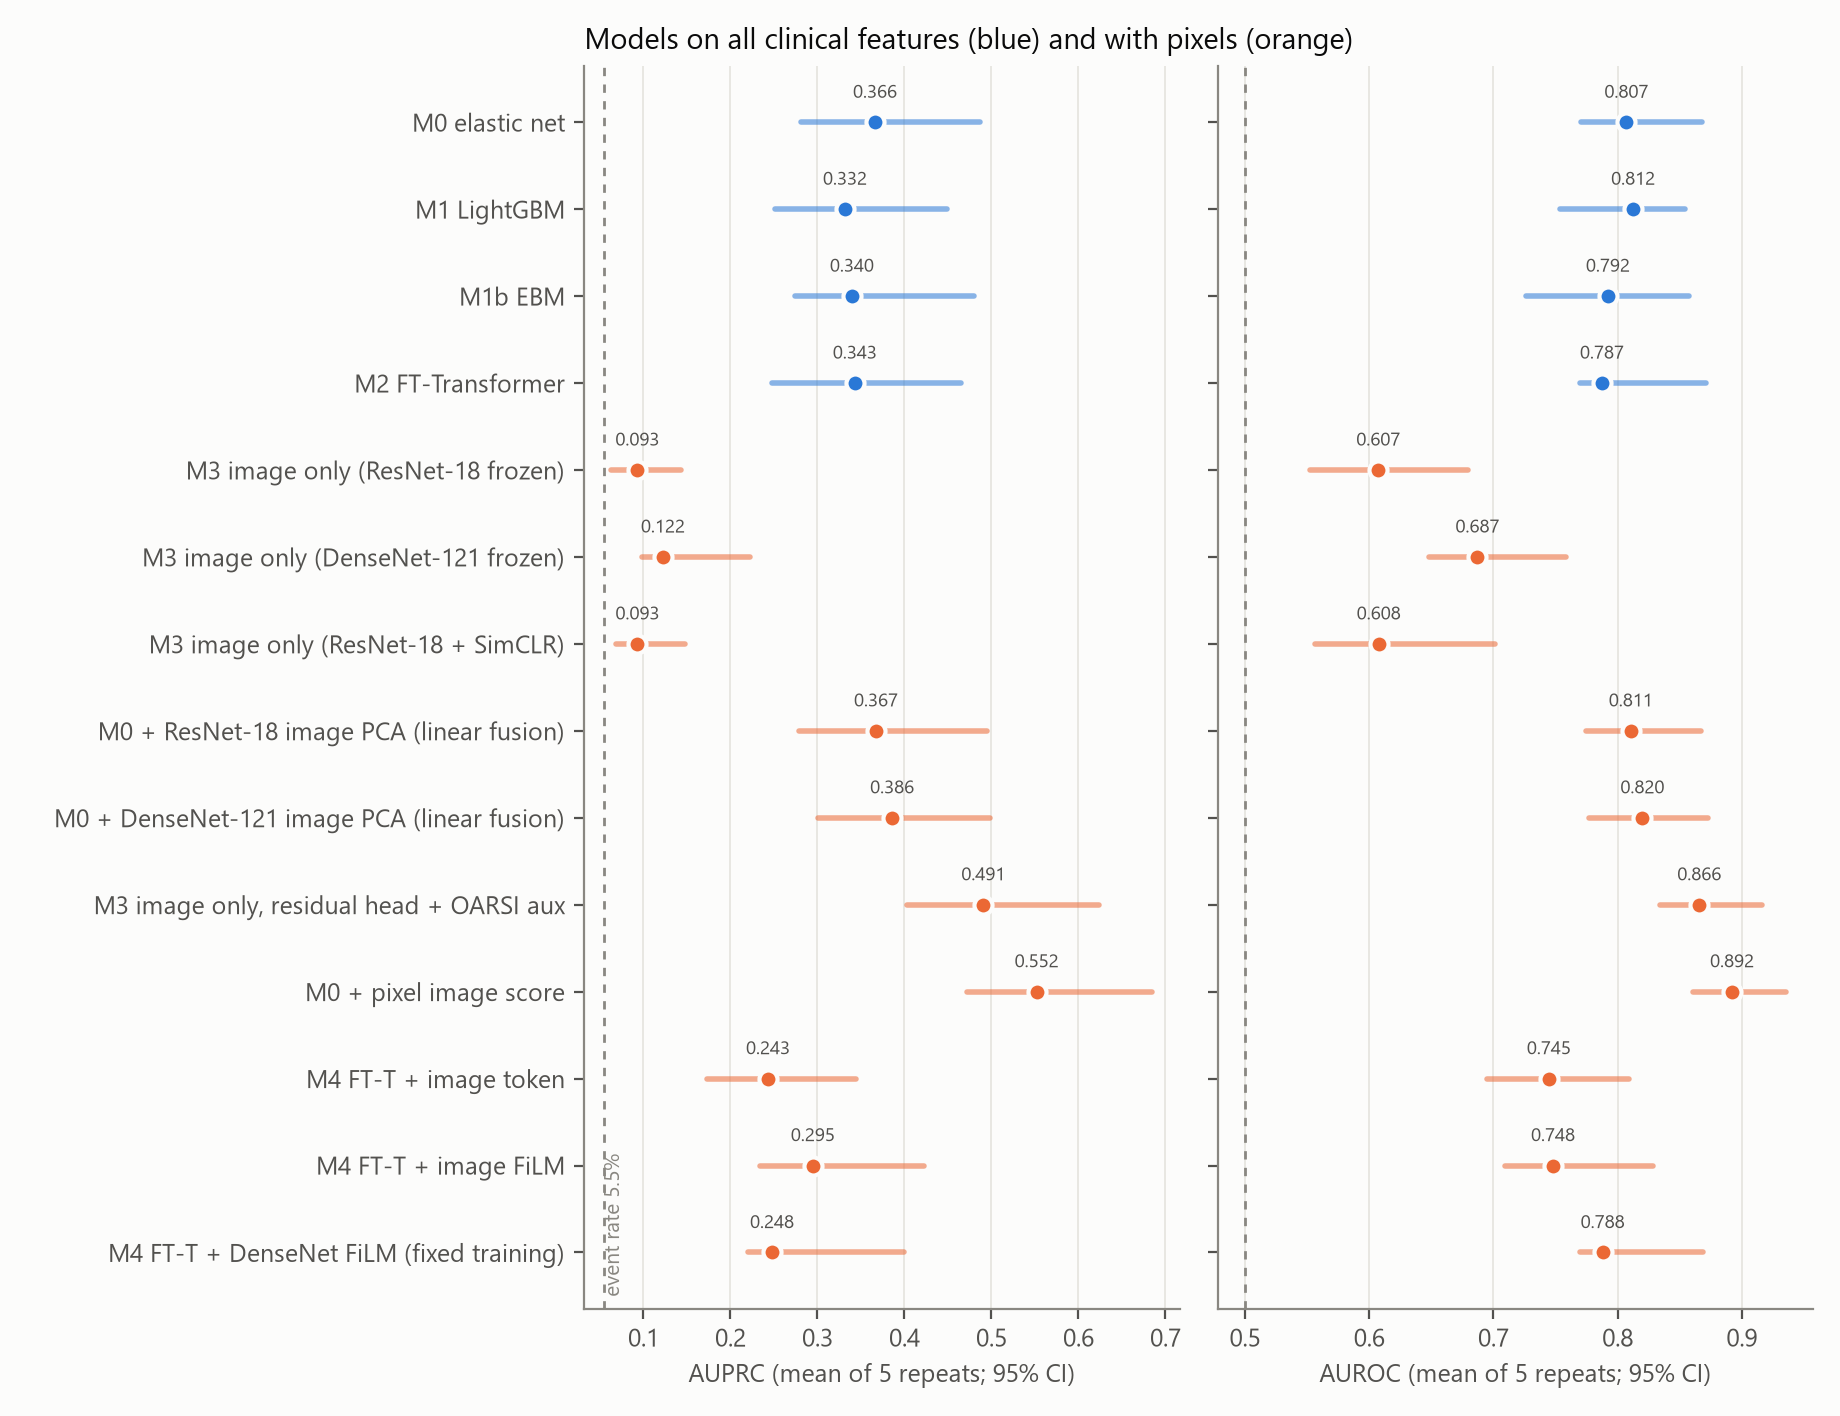
\includegraphics[width=\linewidth]{res_models_DESCLB.png}
  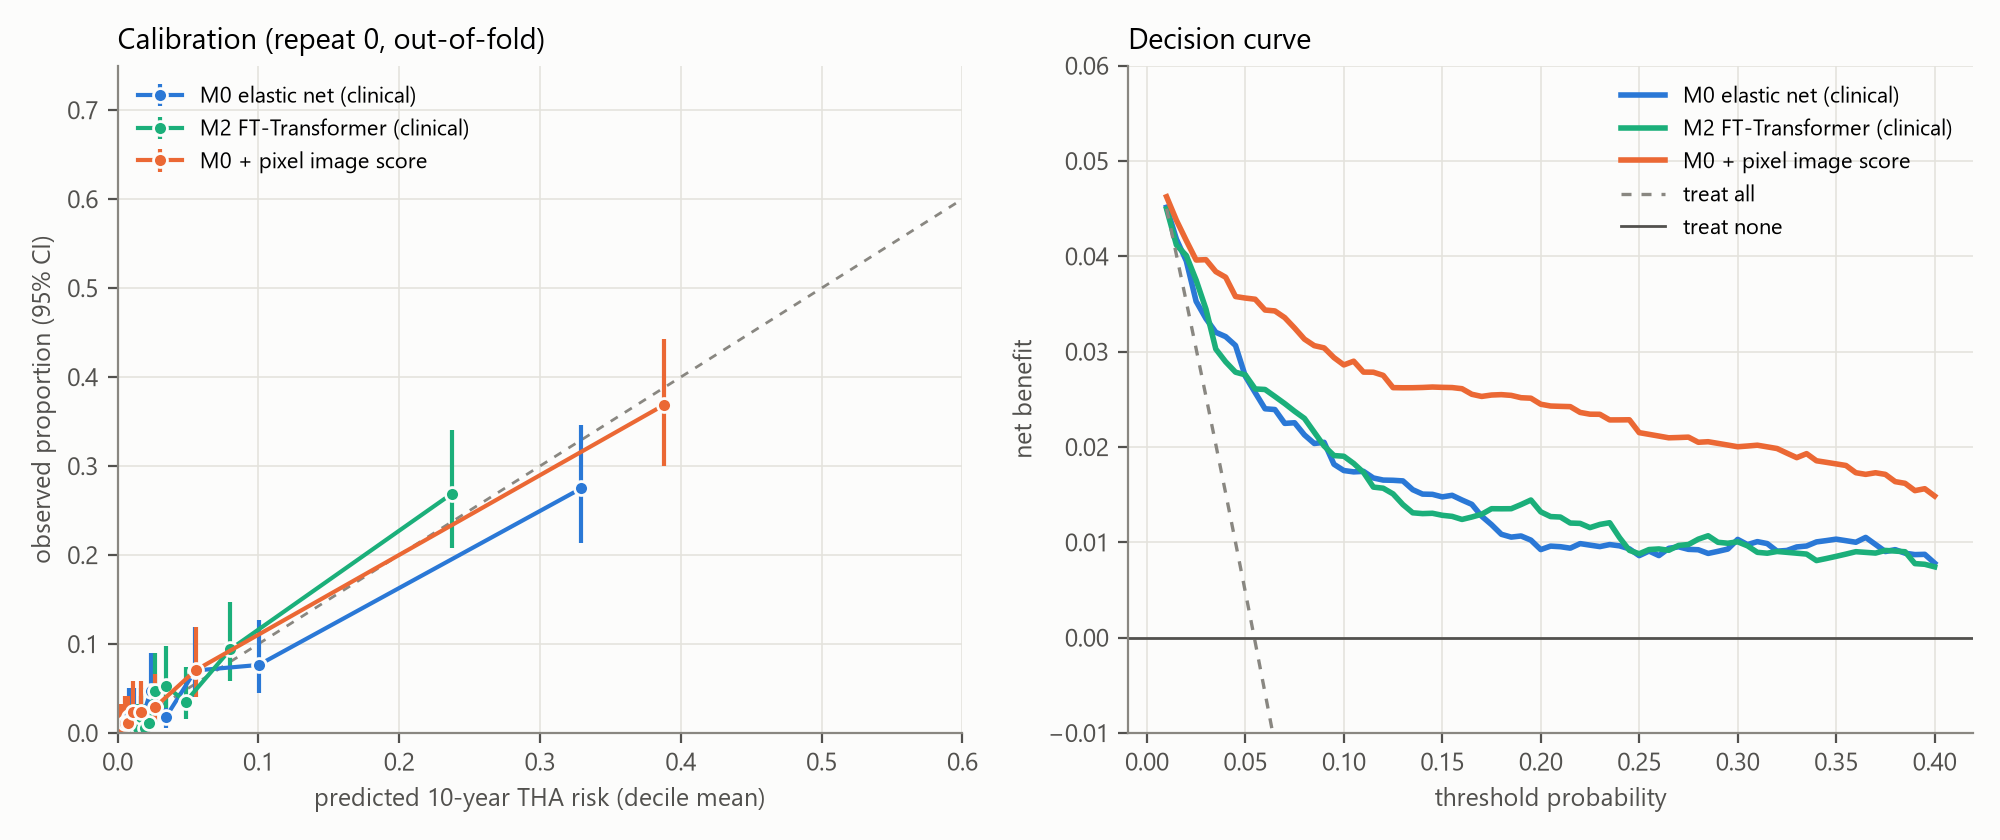
\includegraphics[width=\linewidth]{res_calibration_dca.png}
  \caption{\textbf{Model comparison, calibration and clinical utility.} Top: AUPRC and AUROC of all models on the full
  clinical set (blue) and with image information (orange); the dashed line is the event rate. Bottom: decile calibration
  and decision curves (repeat-0 out-of-fold predictions after Platt recalibration).}
  \label{fig:models}
\end{figure}

\paragraph{}
The FT-Transformer matched M0 in discrimination ($\Delta$AUPRC $-0.030$, $-0.082$ to $0.026$; AUROC 0.787) and had the
best calibration slope (1.04, against 0.84 for M0). Its discrete-time head gave usable 2- and 5-year rankings (AUROC 0.90
and 0.85). The training fixes changed stability more than level: the per-repeat SD of AUPRC fell from 0.060 to 0.024
(Fig.~\ref{fig:hpo}c). BatchNorm in place of LayerNorm gave AUPRC 0.337 (SD 0.017), so it was not adopted. The fusion
model's calibration slope was 0.79. At a 10\% decision threshold its net benefit was 0.029, against 0.018 for M0
(Fig.~\ref{fig:models}).

\paragraph{Image model.}
On pixels alone, frozen pooled features reached AUPRC 0.122 (0.098--0.222; AUROC 0.687), and a linear head on them
0.228 (AUROC 0.769). The residual head with auxiliary targets reached 0.491 (0.403--0.624; lift 9.0) and AUROC 0.866
(0.834--0.917), $+0.362$ (0.254--0.464) over
the frozen model. Most of the gain came from the spatial residual stage (linear $\to$ residual: $+0.268$,
0.154--0.362). Without auxiliary targets, discrimination was unchanged ($\Delta+0.011$, $-0.046$ to $0.072$), and the
calibration slope was 0.95 against 0.84. The supervised head recovered OARSI items better than frozen embeddings (KL
$\rho$ 0.31~$\to$~0.45; superior femoral osteophytes 0.24~$\to$~0.40).

\paragraph{}
In the attention maps (Fig.~\ref{fig:attention}), correctly ranked THA hips drew weight on the superolateral joint
space. False positives were mostly KL 1--2 hips with attention in the same place. Missed THA hips looked near-normal
(KL 0--1), and their attention fell on the medial pelvic wall. Quantified on repeat 0, THA hips ranked in the top 10\%
placed 69\% of their attention inside a disc of 1.6 head radii around the head centre. Missed THA hips placed 37\%
there, the same as unflagged hips (37\%) and close to uniform attention (31\%). Restricting attention and pooling to
that disc did not change performance (image only $\Delta$AUPRC $+0.004$, $-0.043$ to $0.056$; fusion $+0.003$,
$-0.026$ to $0.034$). The locator that defines the disc matched the annotated head circles with median Dice 0.82
(IoU 0.69; 279 heads, 3-fold CV).

\paragraph{} AdaBN lowered AUPRC ($-0.076$, $-0.130$ to $-0.027$).
SimCLR continued pretraining changed nothing ($+0.007$, $-0.031$ to $0.040$), even though the forgetting monitors stayed
healthy (probe log-loss 0.225~$\to$~0.213; CKA 0.59). Fusing the frozen embedding as an FT-Transformer token lowered
AUPRC by 0.132 relative to M0. With the cross-fitted pixel logit as the token, the FT-Transformer reached 0.471 (AUROC
0.848), still below the elastic-net fusion ($-0.095$, $-0.150$ to $-0.043$).

\begin{figure}[!tbp]
  \centering
  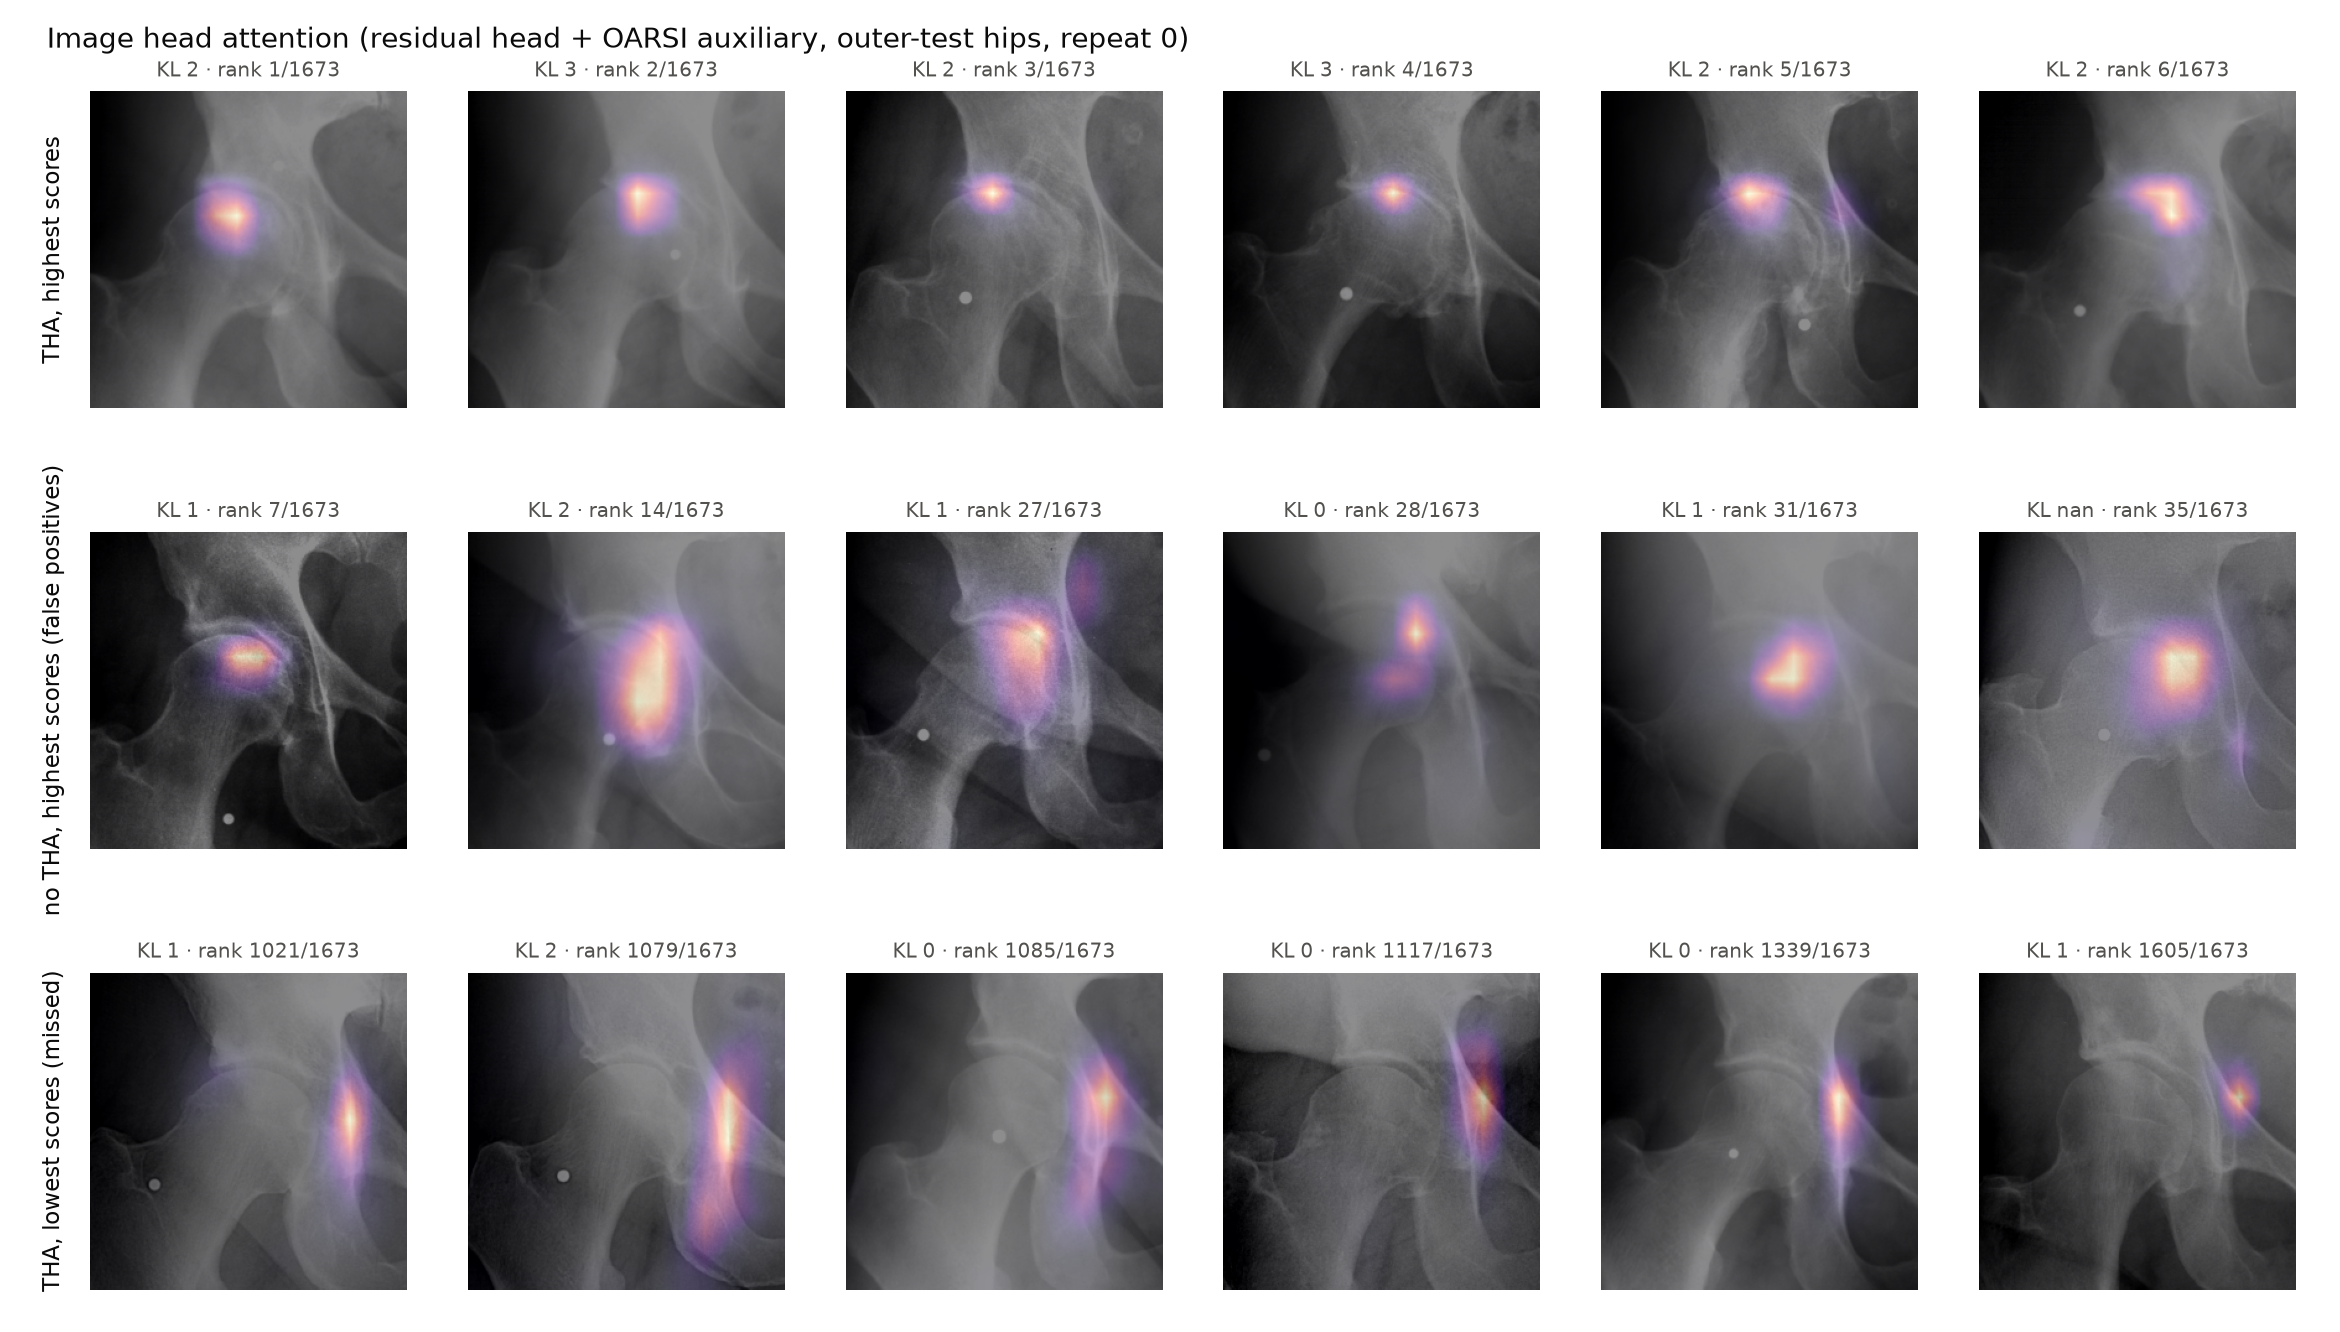
\includegraphics[width=\linewidth]{res_img_attention.png}
  \caption{\textbf{Attention pooling of the image head} on test hips: correctly ranked THA hips, false positives and
  missed THA hips (one outer fold of repeat~0). Weight concentrates on the superolateral joint space in THA hips and
  in KL 1--2 false positives. In missed cases, which look near-normal, it falls on the medial pelvic wall.}
  \label{fig:attention}
\end{figure}

\subsection{Auxiliary analyses}
\label{sec:res-aux}

\paragraph{Interpretability and feature-group ablation.}
The clinical signal lay in examination and symptoms: AUPRC rose from 0.092 (demographics, D) to 0.294 (+E) and 0.392
(+S), while care, social and biochemistry groups added nothing. Dropping E ($-0.081$, $-0.159$ to $-0.003$) or S
($-0.068$, $-0.136$ to $0.000$) hurt most (Fig.~\ref{fig:interp-tab}). FT-Transformer attention was nearly uniform, at most 1.16 times the uniform share. Its
ranking also did not reproduce: two identical reruns put examination tokens first and then demographic tokens first. We
therefore do not interpret it. TreeSHAP was deterministic and ranked comorbidity count, ipsilateral knee pain,
ipsilateral hip pain and internal-rotation ROM highest.

\begin{figure}[!tbp]
  \centering
  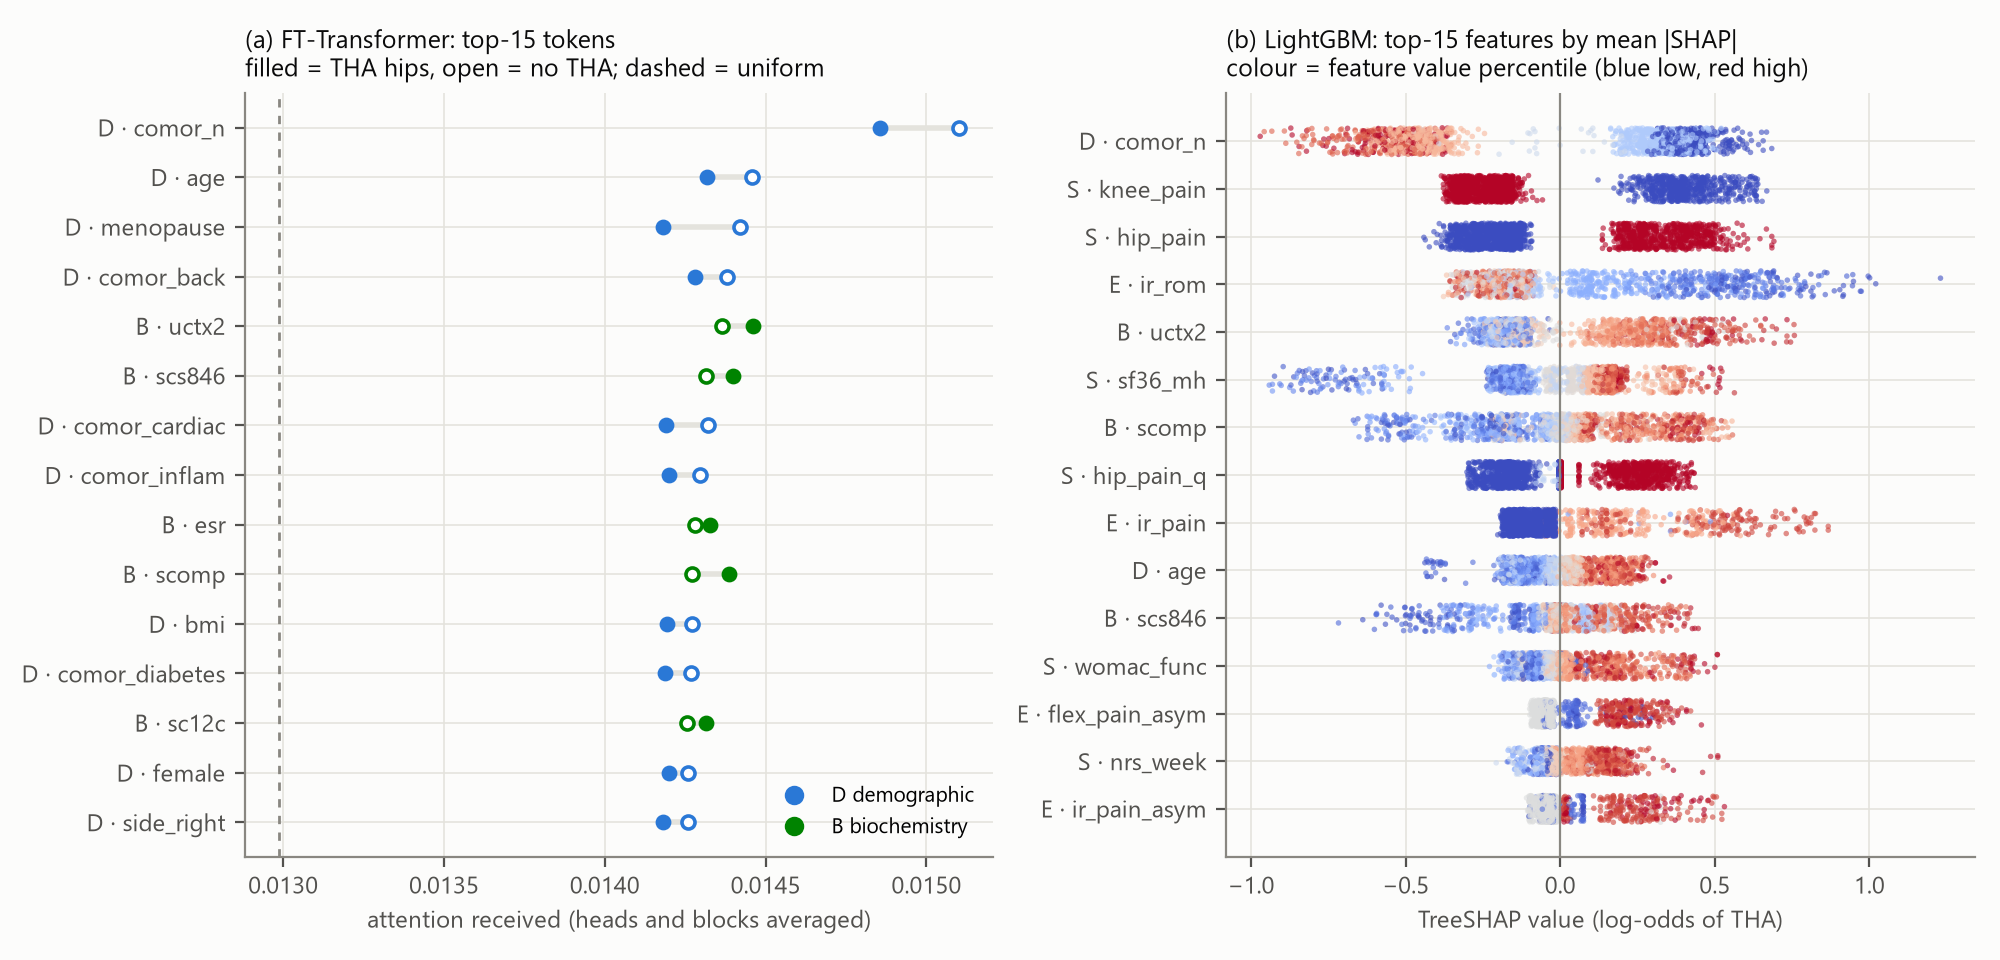
\includegraphics[width=\linewidth]{res_interp_tabular.png}
  \caption{\textbf{Tabular interpretability} (repeat-0 outer test hips). (a) FT-Transformer: attention received per
  token, for THA hips (filled) and the rest (open); the dashed line is uniform attention. All tokens lie within 16\% of
  uniform, and the ranking changed between identical reruns. (b) LightGBM TreeSHAP beeswarm; colour shows the
  feature-value percentile. Higher comorbidity counts and ipsilateral knee pain lower the predicted risk; knee pain marks
  ``bystander'' hips enrolled because of the knee. Hip pain and restricted internal rotation raise it.}
  \label{fig:interp-tab}
\end{figure}

\paragraph{Temporal leakage audit.}
Every input was fixed at $t_0$ (DICOM years 2003--2006; TIFF films in the baseline folder). The readings, the only
inadmissible input, enter no model. Discrimination fell with time to surgery for every model: AUROC was 0.90--0.98 for
THA in years 1--3 and 0.63--0.77 in years 8--10. Without THA in years 1--2, the fusion model reached AUROC 0.876 and
AUPRC 0.455, against 0.785 and 0.271 for M0 ($\Delta$AUPRC $+0.204$, 0.117--0.278). The head trained without readings
matched it ($+0.003$, $-0.062$ to $0.067$). The image score did not predict censoring (AUROC 0.52). One radiograph was
shared by two participants, affecting one THA hip.

\paragraph{Shortcut probes.}
Crop embeddings still identified the pseudo-centre (macro-AUROC 0.90) and the film format (0.93): grey-level handling,
resolution and post-processing remain in the pixels. Removing the centre$\times$format means within training folds
left the outcome probe unchanged (DenseNet 0.725 $\to$ 0.730). The follow-up-group probe dropped from 0.586 to 0.553.
Clinical tables also identified the centre (0.77) and the follow-up group (0.75), because the group was assigned by
symptom severity.

\paragraph{Pseudo-external transport.}
Under leave-one-centre-out validation, M0 kept its discrimination: pooled AUPRC 0.374 against 0.377 internally ($\Delta
-0.003$, $-0.049$ to $0.039$). Calibration did not transport: the intercept ranged from $-1.6$ to $+1.4$ across centres.
Painless hips were over-predicted (intercept $-1.47$; sensitivity 0.72, specificity 0.52 at the source threshold).
Discrimination dropped significantly only from the no-prior-care source to the prior-care target ($\Delta-0.128$,
$-0.220$ to $-0.028$). The image head transported across centres (AUROC 0.858 against 0.876) but lost
0.12--0.13 AUPRC across film formats (single fit, no CI; Appendix~\ref{app:transport}).
